\documentclass[final,t]{beamer}
\mode<presentation>
{
\usetheme{Lankton}
%  \usetheme{Berlin} 
%  \usetheme{Warsaw}
%  \usetheme{Aachen}
%  \usetheme{Oldi6}
%  \usetheme{I6td}
%  \usetheme{I6dv}
%  \usetheme{I6pd}
%  \usetheme{I6pd2}
%  \usetheme{PHI6}
%  \usetheme{PHCVD}
%\usetheme{Icy2}
}
% additional settings
\setbeamerfont{itemize}{size=\normalsize}
\setbeamerfont{itemize/enumerate body}{size=\normalsize}
\setbeamerfont{itemize/enumerate subbody}{size=\normalsize}

%additional packages
\usepackage{times} 
%\usepackage{amsmath,amsthm, amssymb, latexsym}
%\usepackage{exscale} \boldmath 
%\usepackage{booktabs, array}
%\usepackage{rotating} %sideways environment \usepackage[english]{babel}
\usepackage[latin1]{inputenc}
%\usepackage{url}
%\usepackage{hyperref}

%\usepackage{multicol}
%\usepackage{xspace}
\usepackage{natbib}
\usepackage[orientation=landscape,size=a1,scale=0.85]{beamerposter}
\usepackage{Sweave}

% To produce both postscript and pdf graphics, remove the eps and pdf
% parameters in the next line. Set default plot size to 5 x 3.5 in.

%\listfiles
%\graphicspath{{figures/}}
% Display a grid to help align images
%\beamertemplategridbackground[1cm]

\title{Test R Sweave Beamer BeamerPoster Poster on R}
\author[Paul Hurley]{Paul Hurley}
\institute[http://www.paulhurley.co.uk]{http://www.paulhurley.co.uk}
\date[Aug. 16 , 2010]{Aug. 16 , 2010}

% abbreviations
% \usepackage{xspace}
% \makeatletter
% \DeclareRobustCommand\onedot{\futurelet\@let@token\@onedot}
% \def\@onedot{\ifx\@let@token.\else.\null\fi\xspace}
% \def\eg{{e.g}\onedot} \def\Eg{{E.g}\onedot}
% \def\ie{{i.e}\onedot} \def\Ie{{I.e}\onedot}
% \def\cf{{c.f}\onedot} \def\Cf{{C.f}\onedot}
% \def\etc{{etc}\onedot}
% \def\vs{{vs}\onedot}
% \def\wrt{w.r.t\onedot}
% \def\dof{d.o.f\onedot}
% \def\etal{{et al}\onedot}
% \makeatother

%%%%%%%%%%%%%%%%%%%%%%%%%%%%%%%%%%%%%%%%%%%%%%%%%%%%%%%%%%%%%%%%%%%%%%%%%%%%%%%%%%%%%%%%%%%%%%%%%%%%%%%%%%%%

\begin{document}
\Sconcordance{concordance:beamerpostertest.tex:beamerpostertest.Rnw:%
1 76 1 1 11 16 1 1 2 9 0 1 2 6 1 1 4 3 0 1 1 3 0 1 2 1 9 26 0 1 2 3 1 1 %
15 1 16 39 1 2 4 5 1 2 4 65 1 1 8 3 1}

\bibliographystyle{plainnat}
\begin{frame}{}
  \begin{columns}[t]

    %-- Column 1 ---------------------------------------------------
    \begin{column}{0.32\linewidth}

      %-- Block 1-1
      \begin{block}{Summary}
        This is a poster containing text and other things
        This part is the summary.  People might read this
        \\
        These analyses were done on \today, using the following versions of R\citepp{i1609}, Sweave\citep{i1608}, \LaTeX, the
operating system, and add-on packages ggplot2\citep{i1606} and others using Sweave template 
beamerpostertest.Rnw.  It took approx 3.13
 
sec to process.
\scriptsize
\begin{itemize}\raggedright
  \item R version 2.15.1 (2012-06-22), \verb|i686-pc-linux-gnu|
  \item Base packages: base, datasets, graphics, grDevices, methods,
    stats, utils
  \item Other packages: ggplot2~0.9.2.1, plyr~1.7.1, xtable~1.7-0
  \item Loaded via a namespace (and not attached): colorspace~1.1-1,
    dichromat~1.2-4, digest~0.5.2, grid~2.15.1, gtable~0.1.1,
    labeling~0.1, MASS~7.3-21, memoise~0.1, munsell~0.4, proto~0.3-9.2,
    RColorBrewer~1.0-5, reshape2~1.2.1, scales~0.2.2, stringr~0.6.1,
    tools~2.15.1
\end{itemize}\normalsize
      \end{block}

      %-- Block 1-4
      \begin{block}{Tables}
        You can insert tables of data
        \\
% latex table generated in R 2.15.1 by xtable 1.7-0 package
% Wed Sep 19 20:46:20 2012
\begin{tabular}{rrlr}
  \hline
x & y & type & z \\ 
  \hline
  1 & 45.14 & Red & 46.60 \\ 
    2 & 56.81 & Blue & 59.05 \\ 
    3 & 43.03 & Green & 46.12 \\ 
    4 & 51.78 & Yellow & 56.63 \\ 
    5 & 44.31 & Purple & 50.97 \\ 
    6 & 52.85 & Red & 63.66 \\ 
    7 & 70.32 & Blue & 89.95 \\ 
    8 & 61.04 & Green & 87.87 \\ 
    9 & 54.87 & Yellow & 91.63 \\ 
   10 & 47.64 & Purple & 95.27 \\ 
   11 & 37.39 & Red & 91.09 \\ 
   12 & 45.82 & Blue & 144.29 \\ 
   13 & 54.61 & Green & 235.92 \\ 
   14 & 39.66 & Yellow & 212.51 \\ 
   15 & 67.73 & Purple & 625.15 \\ 
   16 & 49.26 & Red & 559.76 \\ 
   17 & 51.89 & Blue & 875.37 \\ 
   18 & 57.40 & Green & 1523.19 \\ 
   19 & 63.40 & Yellow & 2718.07 \\ 
   20 & 33.56 & Purple & 1160.15 \\ 
   \hline
\end{tabular}      \end{block}

%-- Block 1-5
      \begin{block}{Packages}
\begin{figure}[htb]
        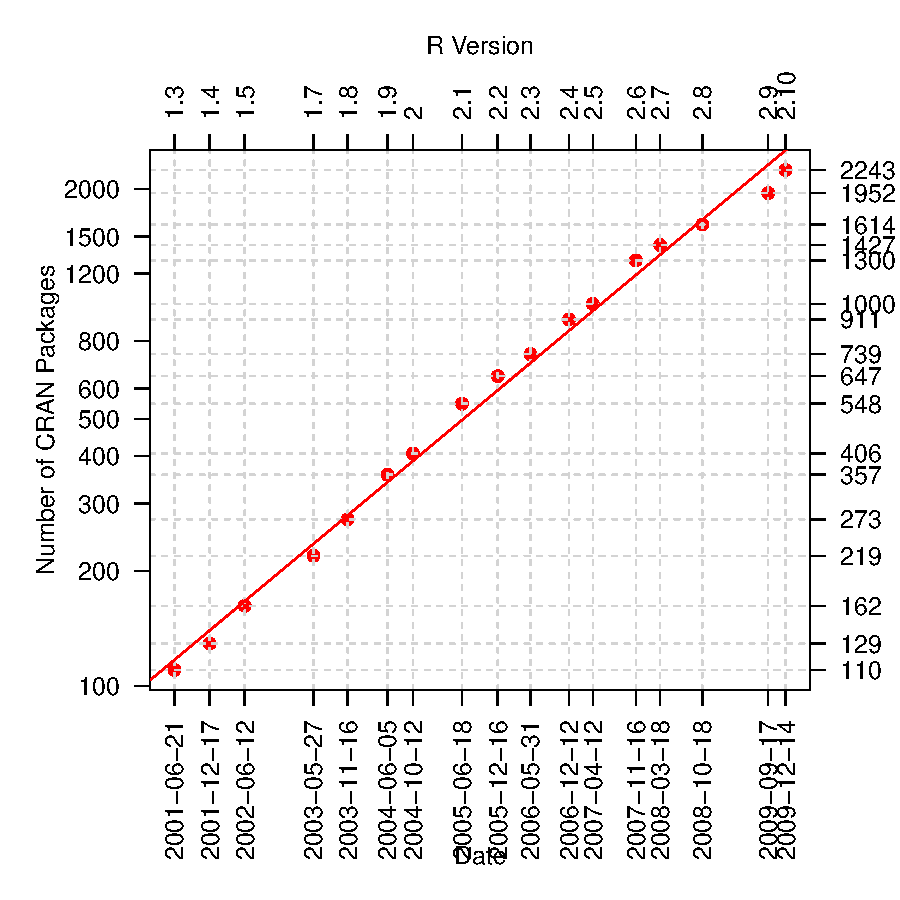
\includegraphics[width=.4\columnwidth]{beamerpostertest-pack}
        \end{figure}
\end{block}

    \end{column}%1

    %-- Column 2 ---------------------------------------------------
    \begin{column}{0.32\linewidth}

      %-- Block 2-1
      \begin{block}{Lists}
        \begin{itemize}
          \item You can make
          \item lists, that
          \item allow people to see quickly
        \end{itemize}
      \end{block}

      %-- Block 2-2
      \begin{block}{Math}
        Include math within the text is as simple as $1+1=2$.
        \\
        \begin{equation}
          a^2 +b^2 = c^2
        \end{equation}
        You can also highlight more important equations like this:
        \begin{equation*}
          \int_0^1\sin(x)+\cos^2(x)+\alpha x~d\!x
        \end{equation*}
        and you can include theorems like this
        \begin{thm}[Rolle]
Let $f\in C^1([x_1,x_2];\mathbb{R})$. If $f(x_1)=f(x_2)$,
then there exists $x_3\in(x_1,x_2)$
such that $f’(x_3) = 0$.
        \end{thm}

      \end{block}

      %-- Block 2-3
      \begin{block}{Pictures}
        \begin{figure}[htb]
        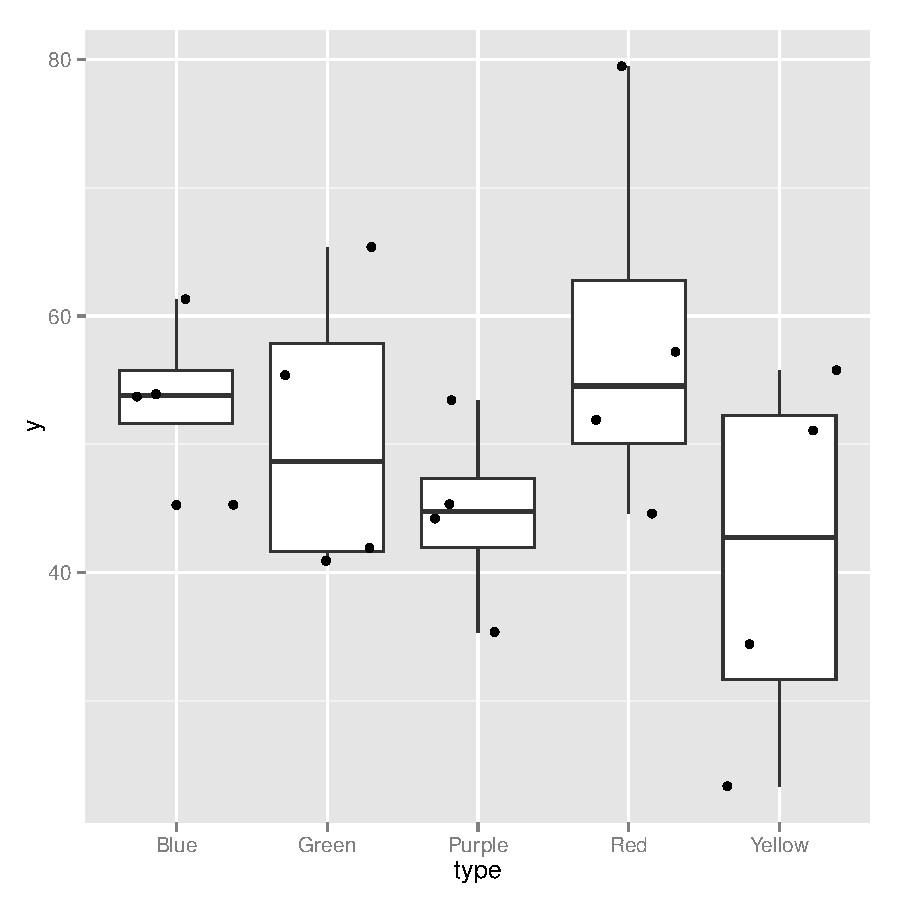
\includegraphics[width=.6\columnwidth]{beamerpostertest-fig1}
        \end{figure}
      \end{block}

  %-- Block 2-4
      \begin{block}{Plots}
        \begin{figure}[htb]
        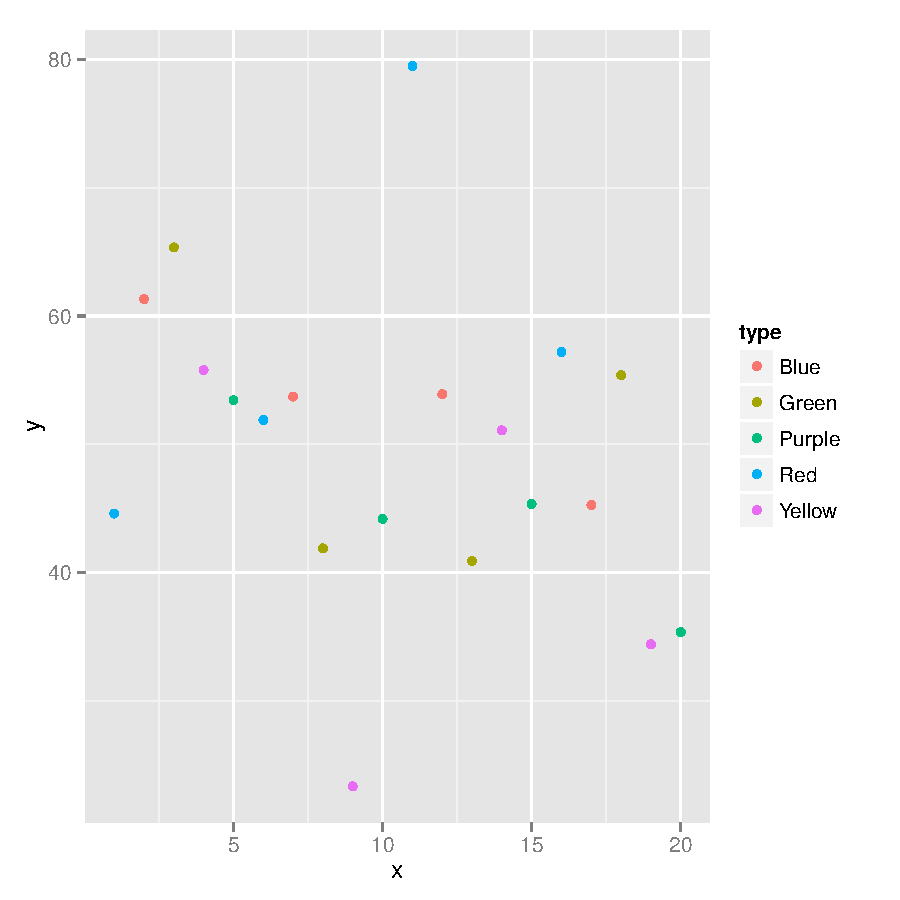
\includegraphics[width=.6\columnwidth]{beamerpostertest-fig2}
        \end{figure}
      \end{block}
      
    \end{column}%2

    %-- Column 3 ---------------------------------------------------
    \begin{column}{0.32\linewidth}

      %-- Block 3-1
      \begin{block}{Experiments}
        Remember to put lots of figures on your poster... Nobody reads anymore!
        \\
        {\tiny tiny size}\\
        {\scriptsize scriptsize size}\\
        {\footnotesize footnotesize size}\\
        {\small small size}\\
        {\normalsize normalsize size}\\
        {\large large size}\\
        {\Large Large size}\\
        {\LARGE LARGE size}\\
        {\huge huge size}\\
        {\Huge Huge size}\\
        
      \end{block}

      %-- Block 3-2
      \begin{alertblock}{Conclusion}
        This is an alert block.  Much less annoying than PowerPoint.  Copy and Paste from your
        document. Overall, a great idea!
      \end{block}

      %-- Block 3-3
      \begin{block}{Logo}
        To change the logo (if you don't want to represent for Georgia Tech).
        Replace the file {\tt logo.png} and with the logo of your choice!
        Make sure the background is black.
      \end{block} 
\begin{block}{So, who uses R ?}
      Well, the buzz around R is growing.
      The popularity of R is growing, with articles appearing in major publications such as
      the New York Times\citep{i1697}, Forbes and InfoWorld\citep{i1698}
      \begin{figure}[htb]
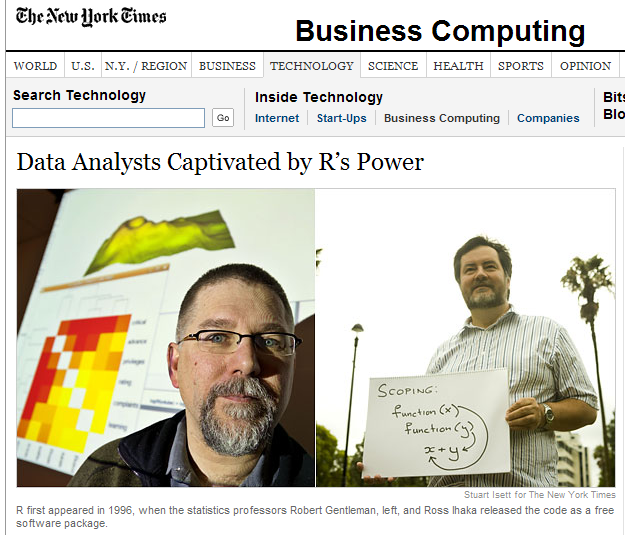
\includegraphics[width=.70\columnwidth]{NYTimes_R_Article.png}
\end{figure}
Today, R is used at many Fortune 500 companies such as Google, Merck, Pfizer, 
Shell and the FDA\citep{i1705} and many others.
    \end{block}
%-- Block 3-4
      \begin{block}{Bibliography}
			% Note: Rsystem reference is defined inside feh.bib. It is a slightly
			% edited version of the output of citation().
			\bibliography{testwhyR}
			\normalsize
		\end{block}
 
 \begin{block}{Creative Commons Sharealike}
 
\includegraphics[width=.15\columnwidth]{cc_attribution_sharealike}
 \end{block}
 
    \end{column}%3

  \end{columns}
\end{frame}


\end{document}


